% !TEX root = ../document.tex
% !TeX spellcheck = pt_BR

% ----------------------------------------------------------
\chapter[Noções de cardiologia]{Noções de cardiologia}
\thispagestyle{empty}
\label{chap:chapter2}
% ----------------------------------------------------------

Neste capítulo são apresentados alguns conceitos fundamentais de cardiologia para a interpretação de ECGs. Também são abordados os padrões do sinal de ECG que correspondem a uma determinada cardiopatia. O livro \cite{Dubin2000} foi utilizado como base para os estudos dos conceitos de cardiologia.

\section{O Ciclo Cardíaco}
O coração é o órgão principal do sistema cardiovascular humano, sendo que o ciclo cardíaco (também chamado batimento cardíaco), é o procedimento pelo qual o coração exerce a sua função de bombeamento de sangue neste sistema. O funcionamento do coração se deve a estímulos elétricos que atuam sobre as células do músculo cardíaco e fazem este se contrair. É através desta atividade elétrica que o sangue é impulsionado do coração para os pulmões, onde ocorre a troca entre gás carbônico e oxigênio, e para todo o resto do corpo, que necessita de oxigênio.

A atividade cardíaca pode ser resumida da seguinte forma. Primeiramente o coração encontra-se em um estado de repouso. Neste estado, as células do miocárdio têm seu interior carregado negativamente e diz-se que elas estão polarizadas (polaridade ``-''). Quando estimuladas por um impulso elétrico, as células despolarizam-se (polaridade ``+'') e ficam então carregadas positivamente. O processo de despolarização faz as células e, por consequência, o miocárdio, se contraírem. Assim, a despolarização pode ser considerada como a progressão de uma onda de cargas positivas dentro das células, estimulando-as a se contrair.

Localizado no átrio direito, encontra-se o Nódulo Sino-Atrial (ou Nódulo SA) que é responsável pela produção dos estímulos elétricos de despolarização. Ele desencadeia uma propagação de cargas positivas ao longo do músculo cardíaco, provocando uma contração quase simultânea dos átrios direito e esquerdo. Esta fase é conhecida como \textbf{sístole atrial}. A sístole atrial impulsiona o sangue na direção dos ventrículos, que estão abaixo no eixo normal do coração. Quando, após um intervalo de aproximadamente 100 ms, a onda de despolarização atinge o Nódulo Atrioventricular (ou Nódulo AV), situado entre os átrios, este transmite o estímulo elétrico aos ventrículos por meio do Feixe Atrioventricular (ou Feixe de His). A pausa entre a emissão do estímulo pelo Nódulo SA e o seu recebimento pelo Nódulo AV é necessária para que o sangue entre nos ventrículos antes deste se contrair.

O Feixe de His é divido em dois ramos, Ramo Direito e Ramo Esquerdo. O Ramo Direito se estende por todo o Ventrículo Direito enquanto o Ramo Esquerdo, pelo Ventrículo Esquerdo. Ambos possuem ramificações chamadas fibras de Purkinje, que são os verdadeiros condutores do estímulo elétrico despolarizante. Tão logo a despolarização seja transmitida às células miocárdicas, os ventrículos se contraem, caracterizando a fase conhecida como \textbf{sístole ventricular}. Após uma certa pausa, os ventrículos repolarizam-se, adquirindo novamente cargas negativas. A fase de repolarização é conhecida como \textbf{repouso entre batimentos}. A figura \ref{fig:heart} ilustra este ciclo dentro da morfologia de um coração humano.

\begin{figure}[ht!]
    \centering
    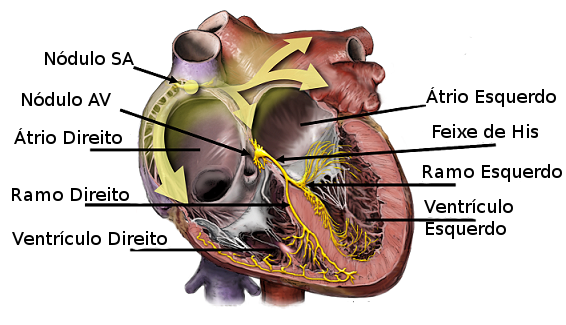
\includegraphics[width=400pt]{figures/chap2-heart.png}
    \caption[Coração e sentido da despolarização]{Coração e sentido da despolarização. Adaptada de \cite{blaufuss}.}
    \label{fig:heart}
\end{figure}

\section{Aquisição do eletrocardiograma}
O ECG é um exame médico que registra a atividade elétrica do coração. As fases do ciclo cardíaco são captadas por um eletrocardiógrafo com o auxílio de eletrodos (ou sensores) cutâneos. Os eletrodos são colocados aos pares no corpo do paciente, de forma que cada configuração de posicionamento dos eletrodos representa uma \textbf{derivação}. Um ECG padrão possui doze derivações, seis delas precordiais (tórax) e seis periféricas (membros). Uma derivação é formada por um eletrodo positivo e um eletrodo negativo, sendo que o ponto de contato do eletrodo positivo define a derivação utilizada.

Quando uma onda despolarização (cargas positivas) se move na direção de um eletrodo positivo instalado na pele do paciente, registra-se uma deflexão positiva no ECG. No caso de um sistema de aquisição com papel milimetrado, a ponteira do eletrocardiógrafo se moverá para cima no traçado. Num sistema de aquisição digital, as amplitudes do sinal na saída do conversor analógico-digital (A/D) se afastarão do valor de referência do conversor no sentido positivo.

Para obter as derivações periféricas, coloca-se eletrodos nos braço direito e esquerdo e na perna esquerda, disposição esta que forma um triângulo, como pode ser verificado a partir da figura \ref{fig:mleads}. A derivação I (DI) é composta por um par de eletrodos dispostos horizontalmente, com o pólo negativo colocado no braço direito e o positivo no braço esquerdo. Na derivação II (DII) o pólo negativo também é colocado no braço direito, porém o positivo vai na perna esquerda. E, finalmente, tem-se a derivação III (DIII) em que o pólo positivo vai na perna esquerda e o negativo no braço esquerdo.

\begin{figure}[ht!]
    \centering
    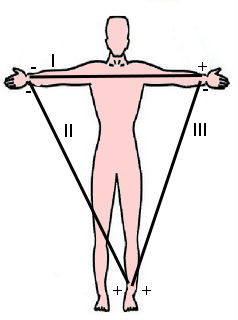
\includegraphics[width=150pt]{figures/chap2-mleads.png}
    \caption[Derivações periféricas: I, II e III]{Derivações periféricas: I, II e III.}
    \label{fig:mleads}
\end{figure}

As outras três derivações periféricas são as chamadas derivações aumentadas, quais sejam: aVR, aVF e aVL. A derivação aVR utiliza um eletrodo positivo no braço direito e um negativo comum (terra) dividido em três pontos de contato: um no braço esquerdo, um no pé esquerdo e outro no pé direito. A aVL é similar, porém com o pólo positivo no braço esquerdo e o negativo comum no braço direito, pé esquerdo e pé direito. Já a aVF é obtida com o pólo positivo no pé esquerdo e o negativo comum no braço esquerdo, braço direito e pé direito. Estas configurações podem ser visualizadas mais facilmente na figura \ref{fig:aleads}.

\begin{figure}[ht!]
 \centering
 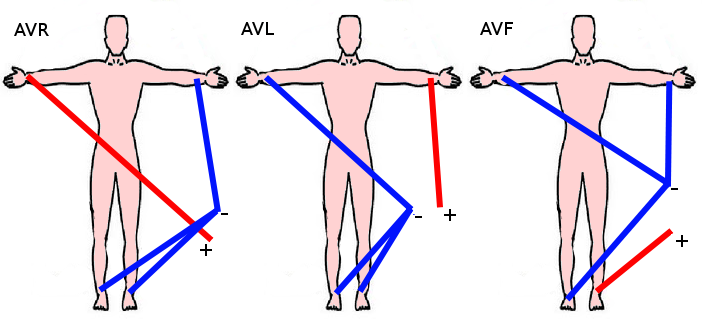
\includegraphics[width=400pt]{figures/chap2-aleads.png}
 \caption[Derivações periféricas aumentadas: aVR, aVL e aVF]{Derivações periféricas aumentadas: aVR, aVL e aVF.}
 \label{fig:aleads}
\end{figure}

As derivações precordiais ou torácicas são obtidas de maneira diferente. Coloca-se eletrodos positivos na parte frontal do tórax, conforme ilustrado na figura \ref{fig:vleads}. O dorso do paciente então é considerado como o pólo negativo da derivação. Na figura \ref{fig:aleads} é possível ver que as derivações V1 e V2 estão localizadas no lado direito do coração; V3 e V4 localizam-se sobre o septo interventricular; por fim, V5 e V6 ficam sobre o lado esquerdo do coração. O intuito dessas derivações é de cobrir totalmente o coração em sua posição dentro da caixa torácica.

\begin{figure}[ht!]
 \centering
 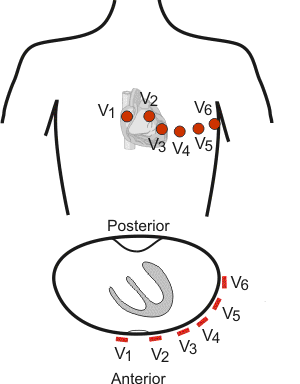
\includegraphics[width=150pt]{figures/chap2-vleads.png}
 \caption[Derivações precordiais: $V_1$, $V_2$, $V_3$, $V_4$, $V_5$ e $V_6$]{Derivações precordiais: $V_1$, $V_2$, $V_3$, $V_4$, $V_5$ e $V_6$. Extraída de \cite{Klabunde2008}}
 \label{fig:vleads}
\end{figure}

Na figura \ref{fig:beat} observa-se um batimento típico registrado em uma derivação de eletrocardiograma. Cinco ondas se distinguem na figura, denominadas pelas letras P, Q, R, S e T. A onda P representa a deflexão causada pela contração atrial (despolarização dos átrios). Já as ondas Q, R e S formam o chamado \textbf{complexo QRS} e representam a despolarização ventricular. Por último, a onda T representa a repolarização ventricular. A repolarização atrial, contudo, dificilmente pode ser visualizada no ECG porque se mistura com o complexo QRS.

\begin{figure}[ht!]
 \centering
 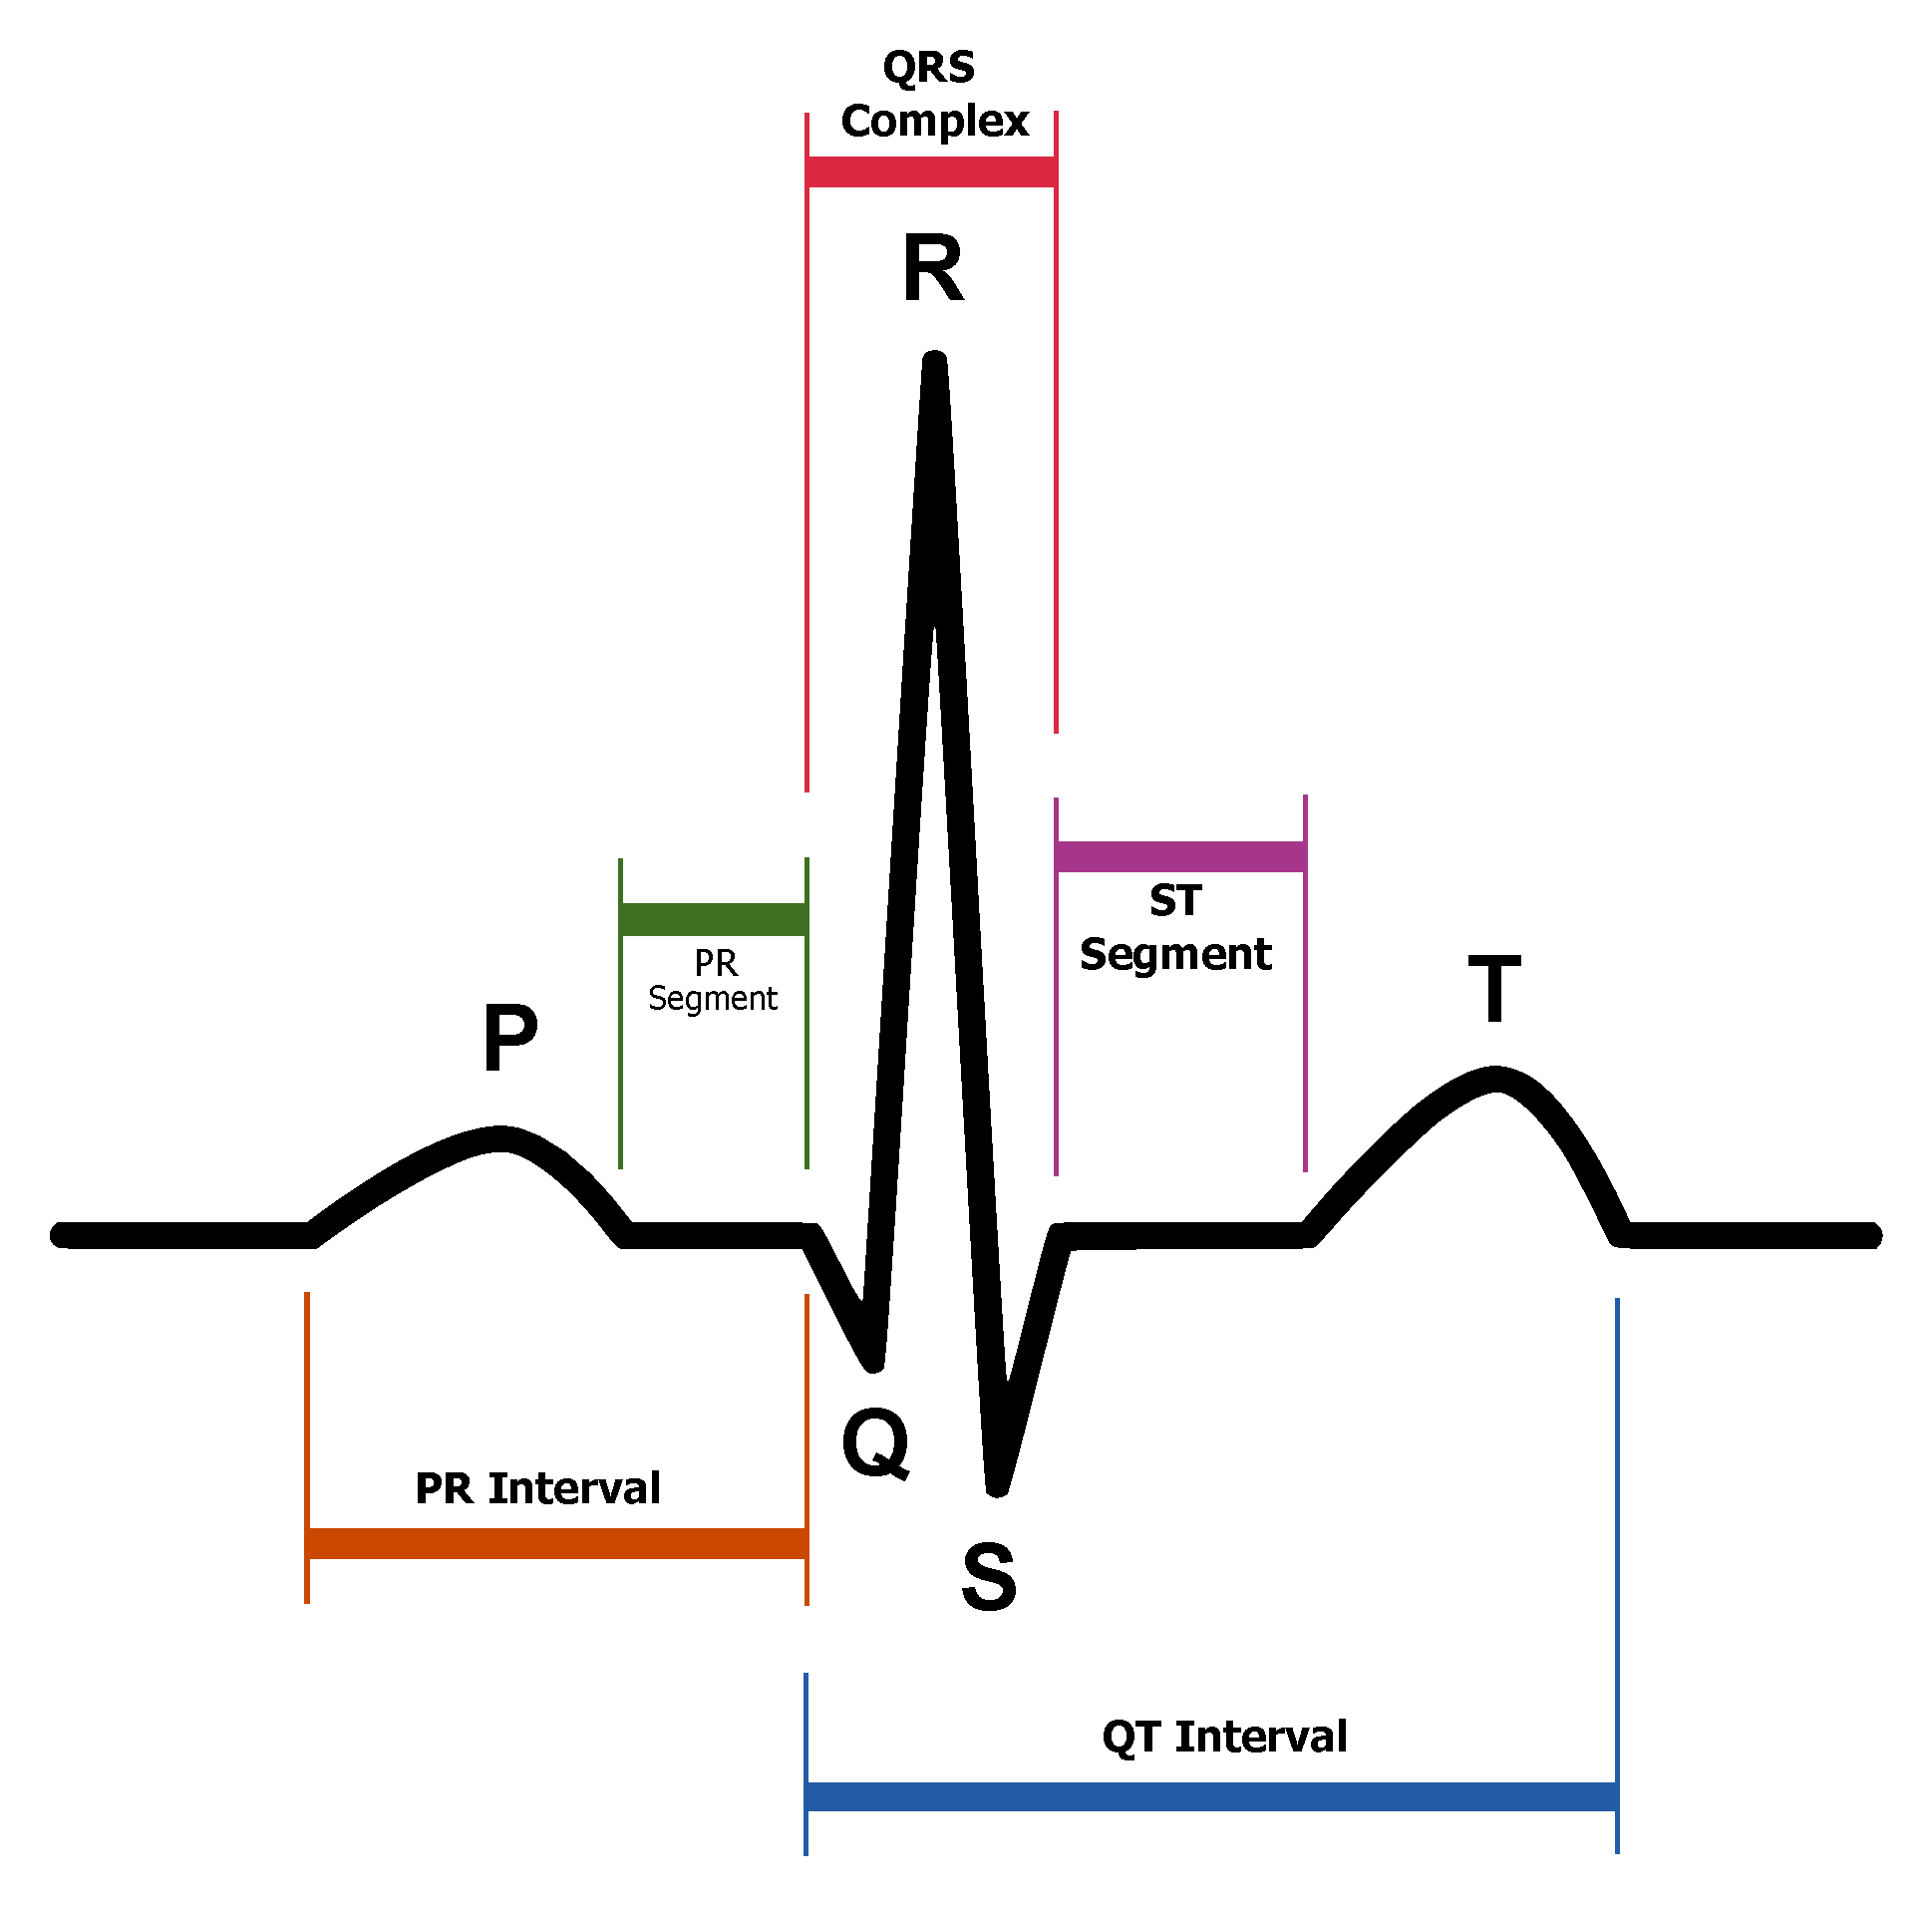
\includegraphics[width=300pt]{figures/chap2-beat.pdf}
 \caption[Ciclo cardíaco típico em um eletrocardiograma]{Ciclo cardíaco típico em um eletrocardiograma. Extraída de \cite{Atkielski2007}}
 \label{fig:beat}
\end{figure}

Ainda na figura \ref{fig:beat}, pode-se ver o chamado segmento PR, entre o fim da onda P e o início da onda Q, representando a pausa que existe entre a emissão do estímulo do Nódulo SA e o recebimento deste pelo Nódulo AV. O segmento ST, por sua vez, representa a pausa existente entre a contração ventricular e a repolarização ventricular. Há ainda o intervalo PR, que indica o tempo decorrido desde o início da despolarização atrial até o seu término. Finalmente, o intervalo QT indica o tempo entre o início da contração ventricular e o fim da repolarização ventricular.

\section{Interpretação do eletrocardiograma}
O ECG nos fornece informações valiosas a respeito da saúde física de um paciente. Em condições normais, um adulto apresenta morfologia de batimento cardíaco nos moldes da figura \ref{fig:beat}. Este padrão varia ligeiramente de acordo com a derivação escolhida, mas pode-se tomá-lo como referência na discussão que segue. Assim sendo, verá-se como uma doença cardíaca acarreta alterações no formato de ondas do ciclo cardíaco, quando analisado por meio do ECG. Ademais, informações como \textbf{frequência}, \textbf{ritmo}, \textbf{eixo}, \textbf{hipertrofia} e \textbf{infarto} podem ser avaliadas a partir do ECG. 

Determina-se a frequência com que os batimentos ocorrem pela distância entre os mesmos no eixo temporal; pode-se então avaliar o ritmo dos batimentos como uma medida qualitativa da variância da frequência cardíaca. Diz-se que o ritmo é normal se a frequência se mantém constante ou quase constante ao longo do intervalo de observação. Caso contrário, diz-se que o ritmo é irregular e tem-se então as chamadas arritmias.

A direção com que se propaga a onda de despolarização do coração é chamada de eixo e é representada por um vetor, o vetor do estímulo elétrico. A partir da análise de várias derivações em conjunto pode-se identificar o eixo, bem como possíveis anormalidades a seu respeito. Também a existência de hipertrofias cardíacas, ou seja, aumento da massa muscular do coração, pode ser observada. Finalmente, é possível averiguar ocorrência de infarto, isto é, morte parcial do músculo cardíaco resultante da oclusão de uma artéria coronária.

Os métodos estudados neste trabalho detectam apenas isquemia cardíaca. Para entender como a isquemia se manifesta no ECG, é necessário conhecer um pouco do sistema cardiovascular e saber que o coração recebe sangue pelas artérias coronárias (figura \ref{fig:arteries}). Quando, por algum motivo, um ramo da artéria coronária se estreita acentuadamente ou fica obstruído, a zona do miocárdio servida por esse ramo deixa de ter irrigação sanguínea adequada.

\begin{figure}[ht!]
 \centering
 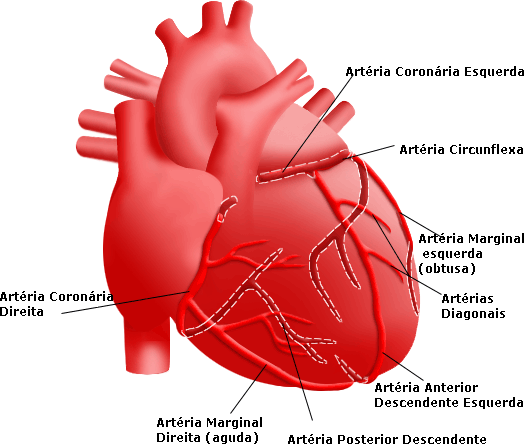
\includegraphics[width=300pt]{figures/chap2-arteries.png}
 \caption[Artérias coronárias]{Artérias coronárias. Extraído de \cite{yale}}
 \label{fig:arteries}
\end{figure}

O ventrículo esquerdo é a cavidade mais espessa do coração, necessitando portanto de maior quantidade de sangue. Assim, no caso de estreitamento das artérias coronárias, o ventrículo esquerdo é o primeiro a sofrer com a redução desse suprimento. É importante saber que o ventrículo esquerdo é em grande parte o responsável por enviar sangue para todas as partes do corpo. Quando parte do ventrículo esquerdo fica infartada, ela se torna eletricamente morta e não responde à despolarização. Consequentemente, ela não se contrai e acaba por prejudicar o bombeamento de sangue do coração. A figura \ref{fig:infarction} ilustra uma possível situação de infarto.

\begin{figure}[ht!]
 \centering
 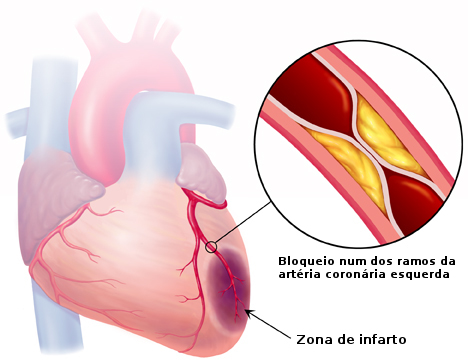
\includegraphics[width=300pt]{figures/chap2-infarction.jpg}
 \caption[Infarto do miocárdio]{Região de infarto do miocárdio. Extraído de \cite{Antipuesto2014}}
 \label{fig:infarction}
\end{figure}

A isquemia cardíaca é a redução do suprimento de sangue ou suprimento abaixo do normal. Ela precede um possível infarto e pode ser identificada no ECG principalmente através de duas características (ou uma das duas): inversão da onda T, podendo variar desde uma onda achatada ou deprimida até uma inversão profunda; e desnivelamento do segmento ST, podendo ser um supradesnivelamento ou um infradesnivelamento.

Nem toda diminuição do suprimento sanguíneo produz um infarto. Ondas T invertidas podem indicar a existência de isquemia sem infarto do miocárdio.  A onda T tipicamente isquêmica é simetricamente invertida. Como as derivações precordiais registram a atividade cardíaca em maior proximidade dos ventrículos, as alterações na onda T serão mais evidentes nessas derivações ($V_1$ a $V_6$). A figura \ref{fig:twave} mostra possíveis variações morfológicas da onda T.

\begin{figure}[ht!]
 \centering
 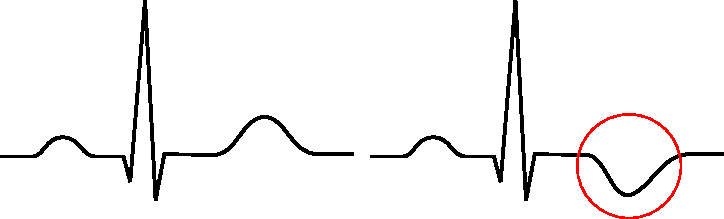
\includegraphics[width=400pt]{figures/chap2-t-waves.pdf}
 \caption[Onda T normal e Onda T isquêmica]{Onda T normal e Onda T isquêmica.}
 \label{fig:twave}
\end{figure}

A isquemia pode causar um lesão no tecido do miocárdio, caracterizando infarto agudo (recente). Para identificar a existência de lesão, analisa-se alteração no segmento ST. A elevação (supradesnivelamento) do segmento ST indica uma lesão e nos dá a certeza de que um infarto é agudo. Em certas situações, como Infarto Subendocárdico e Digitalis, o segmento ST apresenta uma depressão (infradesnivelamento). A figura \ref{fig:stdev} mostra as três variedades de nivelamento do segmento ST.

\begin{figure}[ht!]
 \centering
 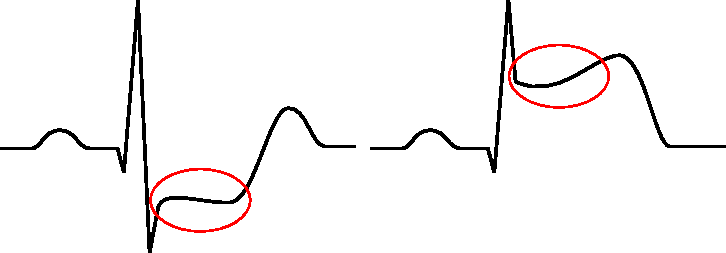
\includegraphics[width=400pt]{figures/chap2-st-segments.pdf}
 \caption[Segmento ST infradesnivelado e supradesnivelado]{Segmento ST infradesnivelado (1) e supradesnivelado (2).}
 \label{fig:stdev}
\end{figure}


\section{Resumo}
O ciclo cardíaco é um fenômeno fisiológico vital para os seres humanos. Essencialmente, tem-se que o Nódulo Sino-Atrial origina uma onda de despolarização (cargas positivas), consequente sístole atrial e, por meio do feixe de His, sístole ventricular. Após um período de repouso, átrios e ventrículos repolarizam-se (adquirem cargas negativas) e tornam-se capazes de iniciar um novo ciclo. É através desta atividade que o sangue circula em direção aos pulmões e para todo o resto do corpo, voltando ao coração após a troca gasosa e de nutrientes.

O exame de ECG registra as etapas do ciclo cardíaco por meio de derivações precordiais e/ou periféricas, formadas por um par de eletrodos cutâneos com cargas elétricas opostas. As derivações registram deflexões que representam cada uma das fases do ciclo, quais sejam: onda P, que é a deflexão causada pela contração atrial; as ondas Q, R e S, que formam o chamado complexo QRS e representam a contração ventricular; e a onda T, que representa a repolarização ventricular. A partir desse registro, é possível identificar informações como frequência cardíaca, ritmo, eixo, hipertrofia e infarto. 

Especialmente, estamos interessados em identificar isquemia cardíaca, que é a redução do suprimento de sangue ao coração. A falta de irrigação sanguínea adequada ao coração, sobretudo ao ventrículo esquerdo, antecede um possível infarto e pode ser identificada pela ocorrência de inversão da onda T ou desnivelamento do segmento ST. É com base nessas informações que se consegue diagnosticar a isquemia a partir do ECG.
